%\begin{figure}[t]
%\vspace{-0.5in}
%\centering
%\psfig{figure=figures/plots/runtimeFinal.eps,width=5.5in} }
%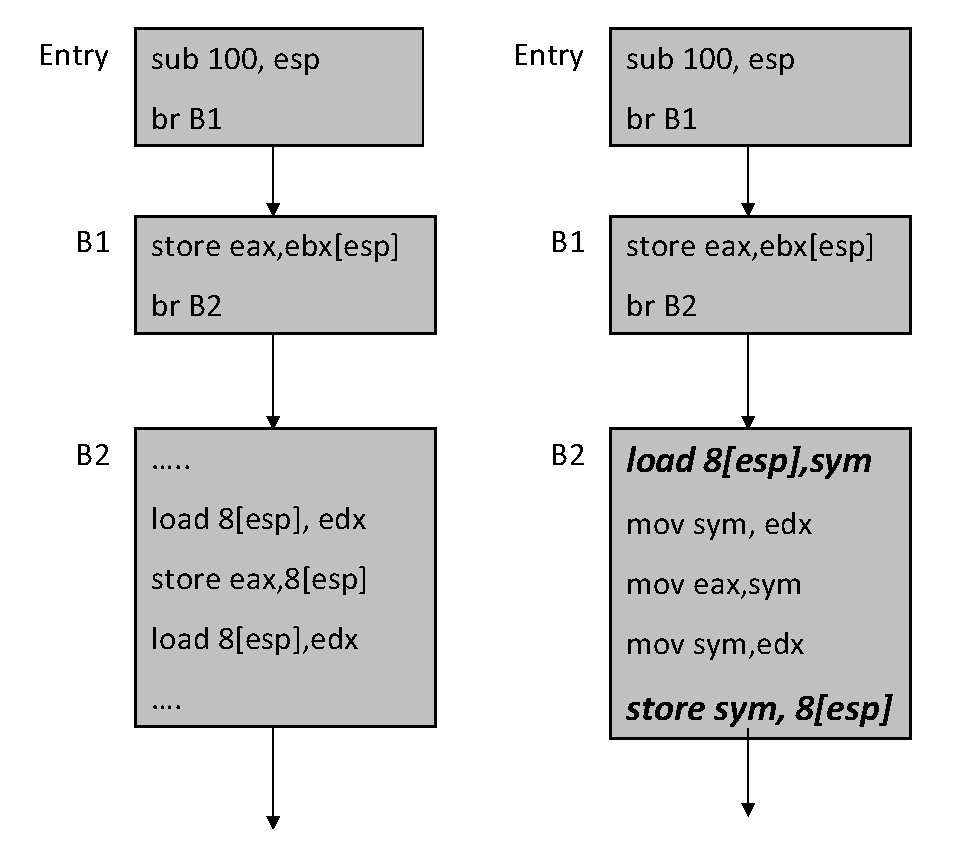
\includegraphics [width=0.5\linewidth] {figures/EPS/cfgex.eps} 
%\tiny{
%\caption { \textit{Stack layout in a binary}}
%}
%\label{fig:stack-layout}
%\end{figure}

\begin{figure}[b]
{
\vspace{-2ex}
\centering
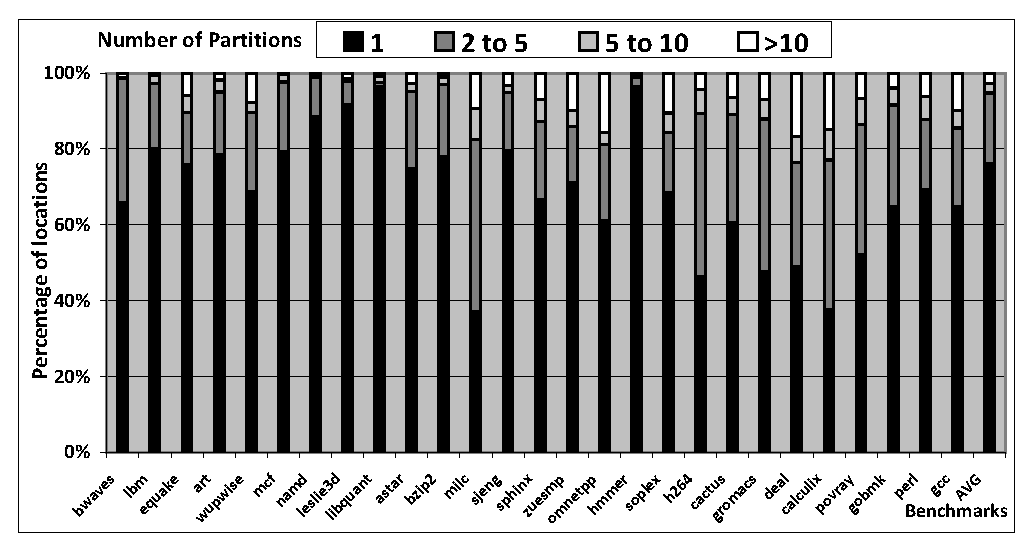
\includegraphics[width=0.8\linewidth]{figures/EPS/partition-visualization-2.eps}
%\vspace{-3ex}
\caption{\textit{Partition algorithm visualization }}
\label{fig:PartResult}
}
%\hfill
\vspace{-3ex}
\end{figure}




%\begin{figure}[t]
%{
%\centering
%\begin{minipage}{.6\linewidth}
%{
%\centering
%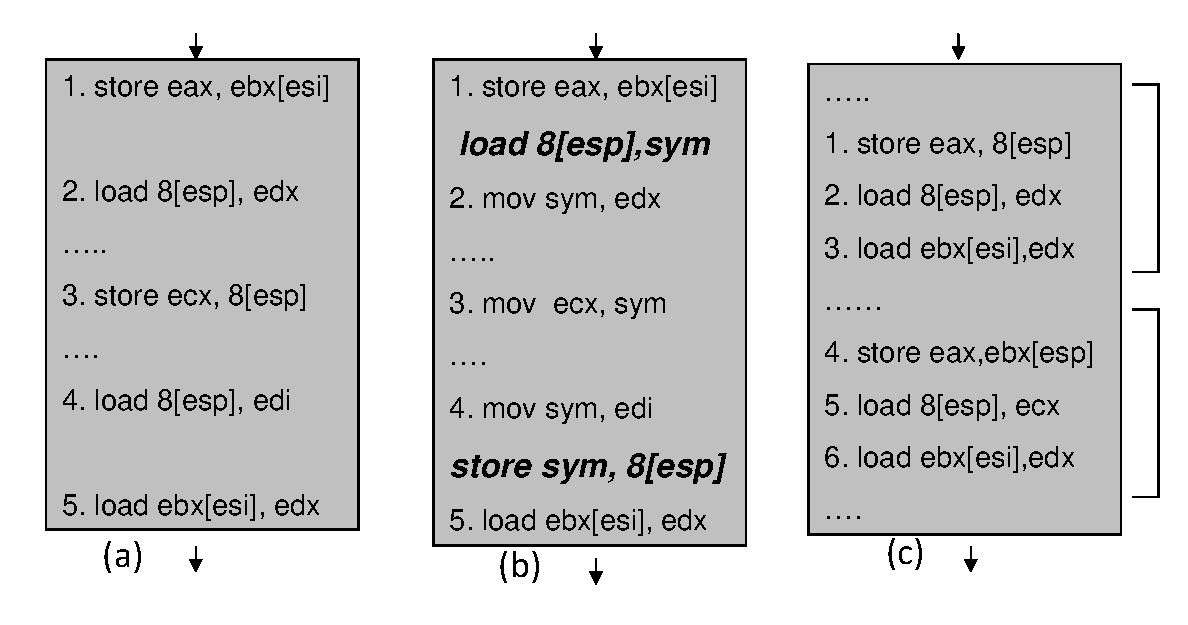
\includegraphics[width=0.5\linewidth]{figures/EPS/pathcfg.eps}
%\caption{\textit{Path dependent promotion. Second operand in the instruction is the destination of the instruction. }}
%\label{fig:PromExample}
%}
%\vspace{-0.1in}
%\end{minipage}
%%\hfill
%\begin{minipage}{0.3\linewidth}
%{
%\centering
%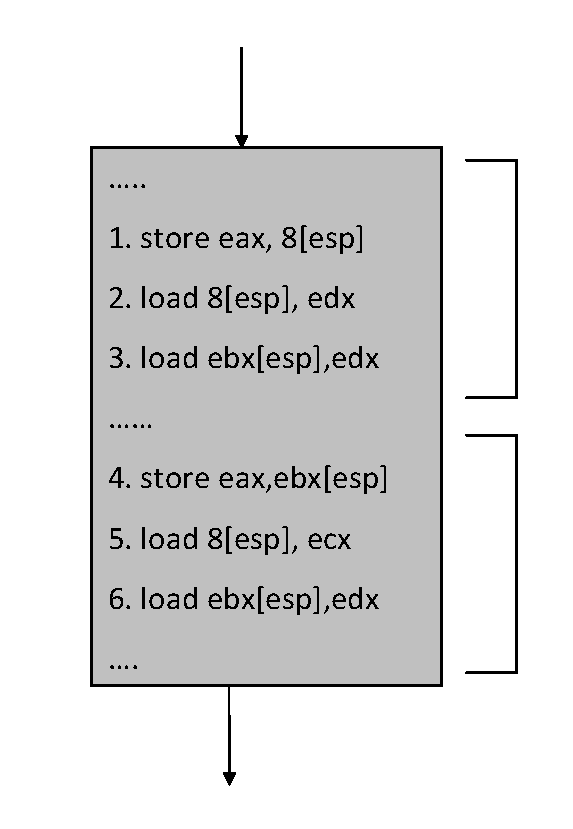
\includegraphics[width=0.3\linewidth]{figures/EPS/partitioncfg.eps} 
%\caption{\textit{Motivation for partition}}
%\label{fig:PartExample}
%}
%\vspace{-0.1in}
%\end{minipage}
%}
%\vspace{-0.2in}
%\end{figure}
